% -------------------------------------------------------------------------------
% Name:         main.tex
% Author:      	@utahkaA (Twitter, GitHub, and so on...)
% Created:     	Jun 23rd, 2016
% Last Date:   	Jun 23rd, 2016
% Note:         xxxxx
% -------------------------------------------------------------------------------
\documentclass[a4jsme]{jsmepaper}
\usepackage[dvipdfmx]{graphicx}
\usepackage{fancyhdr}
\usepackage{epic,eepic}

\thispagestyle{fancy}
\lhead{\gt \normalsize 2016年度前期ゼミナール中間報告書}
\renewcommand{\headrulewidth}{0pt}
\cfoot{\thepage}
%\pagestyle{empty}

\jtitle{ゼミナール報告書テンプレに関するサンプル}
\etitle{Seminar template in OKLAB}
\jauthor{
  1326xxx\ \ 
  氏名
}
\eauthor{
  Write your name in roman letters
}
\jaffiliation{
  & 指導教員:大川 茂樹
}
% 著者の所属の英文
% \eaffiliation{
%     $^{*3}$  □□ Engineering, □□ University \\
%     address
%     }
% 主著者の所属の英文
%\email  {□□□□@□□□□□□}
% 原稿の事前講演など。無い時はコメントアウト
% \presentation{    年 月  日 }
% 原稿受付日(省略すると本日)
\date{\today}
% 英文の概要
\abstract{
  xxxxxxxxxxxxxxxxxxxxxxxxxxxxxxxxxxxxxxxxxxxxxxxxxxxxxxxxxxxxxxxxxxxxxxxxxxxxxx
\abind
  xxxxxxxxxxxxxxxxxxxxxxxxxxxxxxxxxxxxxxxxxxxxxxxxxxxxxxxxxxxxxxxxxxxxxxxxxxxxxx
}
% キーワード
\keywords{xxxx,yyyy,zzzz}

\begin{document}
\maketitle
\thispagestyle{fancy}

\section*{はじめに}
\section{実験装置および方法}

画像は,eps とか使うより,png でいいと思います.
\begin{figure}[htbp]
  \begin{center}
    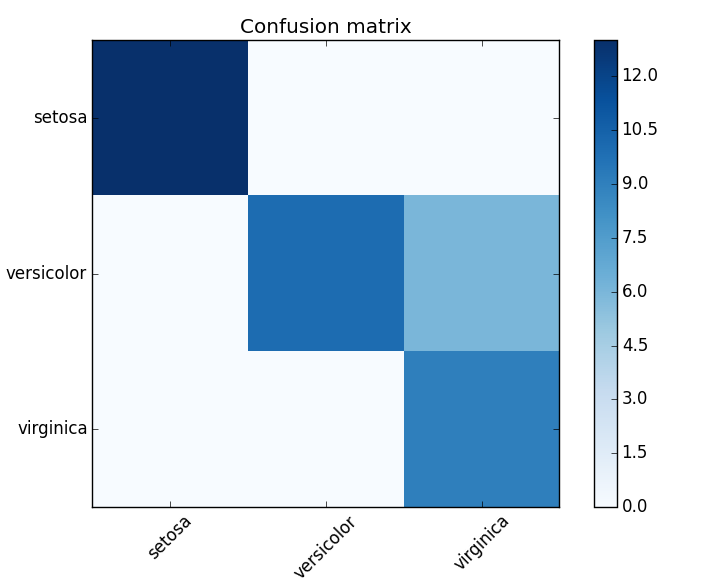
\includegraphics[width=7cm]{img/iris_confusion_matrix.png}
    \caption{アヤメの品種を識別した際の混合行列}
    \label{fig:one}
  \end{center}
\end{figure}

\section{第2章です。}
\subsection{第2章第1節です。\\}

実験にあたり,
\section{第3章です。}
\subsection{第3章第1節です。}
\subsection{第3章第2節です。}
\section{第4章です。}
\section*{おわりに}

{\small
\begin{thebibliography}{99}
  \bibitem{□□□□}
    □□著者□□, □□著者□□,
    {\it □□□書籍題名□□□},
    □□出版社□□, (□発行年□),
    pp.□□--□□
  \bibitem{□□□□}
    □□著者□□, □□著者□□,
    {\it □□□論文題名□□□},
    ``□□雑誌名□□'',
    □巻□,□号□, (□発行年□),
    pp.□□--□□
\end{thebibliography}}

\clearpage
\end{document}
